\section{Introduction}
\label{sec:introduction}
Kitting is a critical aspect of industrial automation that involves organizing and placing 3D parts into complementary cavities. This process saves time on the manufacturing line and frees up space to reduce shipping and storage cost. Automating kitting requires picking and rotating a part to a desired position and orientation, then inserting it into a cavity that loosely conforms to the object geometry. However, this process is a great challenge, and in industry, most kitting % has not been automated and is mostly manual. [removed -KG 3/18]
is performed manually.

\begin{figure}[t]
  \centering
  %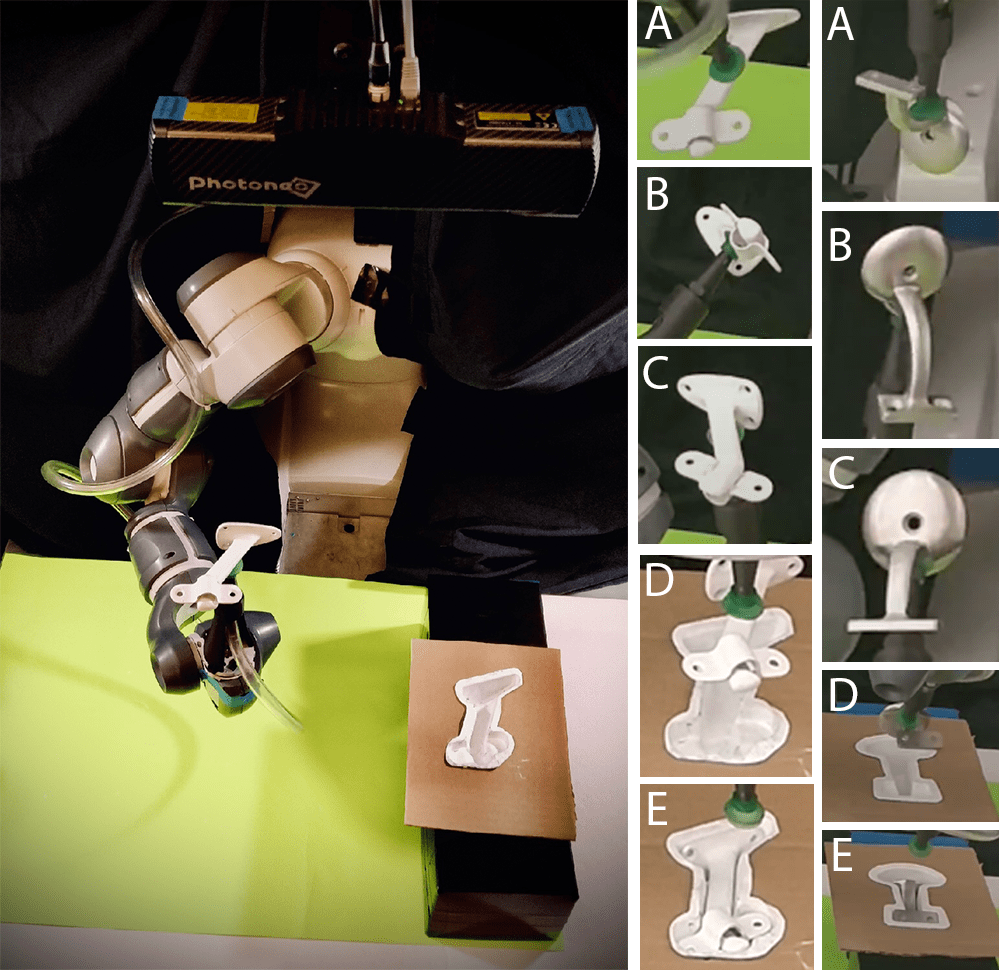
\includegraphics[width=0.48\textwidth]{figures/Fig1_Final.png}
  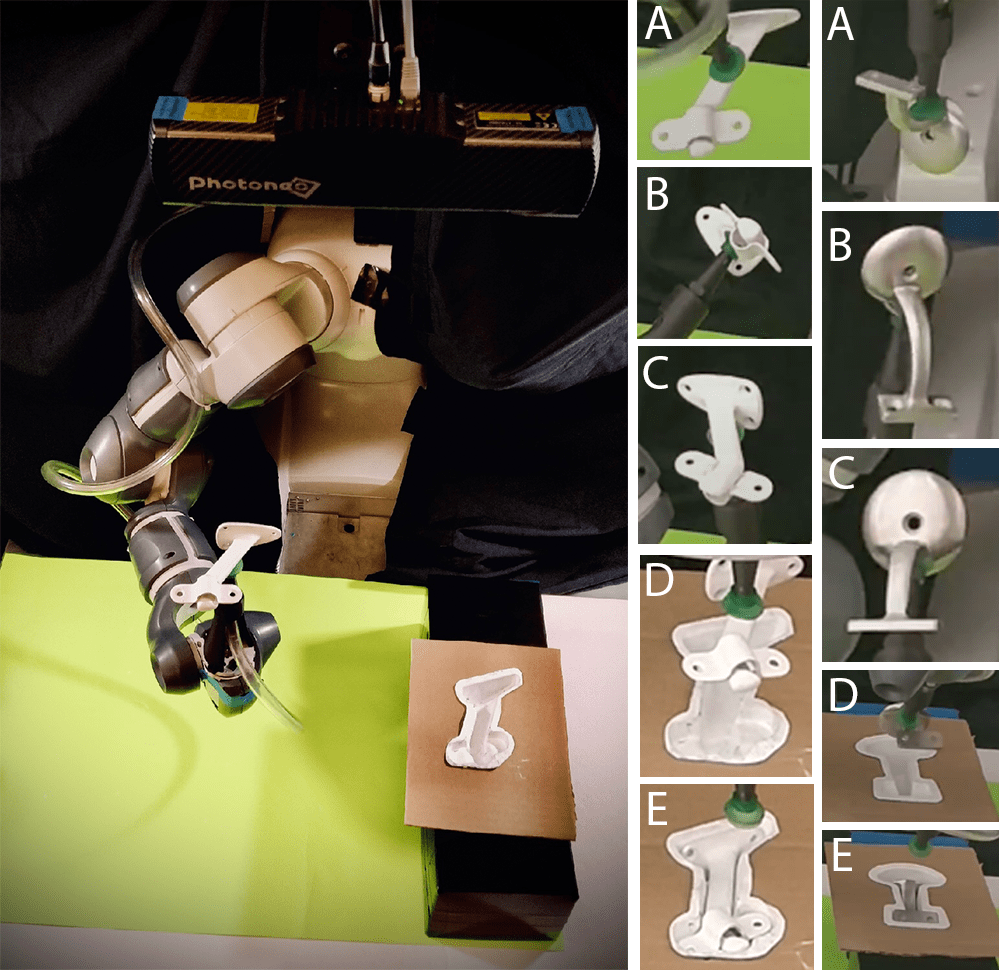
\includegraphics[width=\columnwidth,trim=0 0 187 0, clip]{figures/Fig1_Final.png}
  \caption{Physical experiments using the ABB YuMi and a Photoneo depth camera. (Left) A suction gripper holds the handrail bracket, an object unseen during training time,
  %from the top in a pose unsuitable for kitting. A 
  near the kitting cavity. % target is shown on the bottom right.
  Kit-Net orients the handrail bracket
  %(middle) and the ornamental handrail bracket (right) 
  for insertion into the cavity through 5 steps. A) Starting state. B) Rotate the object by 180\degree~to face the 3D camera and minimize occlusion from the gripper. C) Iteratively orient the object into a goal configuration. %using depth images of the kitting cavity
  D) Rotate by 180 degrees and align centroids of the object and cavity to prepare for insertion. E) Insert and release.}
  \label{fig:splash}
\end{figure}

Given a 3D CAD model of the object to be inserted and the desired object pose, one approach is to directly estimate the object pose and the transformation to the desired pose~\cite{ChoyDeepGlobal, xiang2017posecnn}. However, CAD models may not be available for all objects to be kitted and are time consuming to create for every object, motivating an algorithm that can kit previously unseen objects without requiring such models. Prior work has considered kitting objects without models, 
but has focused on $SE(2)$ transforms (1D rotation and 2D translation) for extruded 2D polygonal objects~\cite{Zakka2020Form2FitLS,zeng2020transporter}. 
% In contrast, we aim to estimate 3D rotations for previously unseen objects such that they can be matched to and inserted into a novel cavity.

% However, achieving a desired orientation often requires implicit knowledge of the object's current and desired orientation. Prior work on estimating object orientation has primarily focused on purely geometric algorithms or explicit pose estimation from sensed visual data \AB{cite} These approaches have made it possible for robots to accomplish a variety of complex manipulation tasks~\AB{cite}, but require knowledge of object geometry or do not generalize well to unseen objects~\AB{cite}.

We formalize the problem of rotating and translating a novel 3D object to insert it into a novel kitting cavity and present Kit-Net,
%an algorithm [replaced -KG 3/18]
a framework for inserting previously unseen 3D objects with unknown geometry into a novel target cavity given depth images of the object in its current orientation and a depth image of either a flipped (convex) or standard (concave) target cavity. Kit-Net extends prior work from~\citet{CASE_Orienting}, which used simulation and self-supervision to train a deep neural network to directly estimate 3D transformations between the two depth images. Given the trained deep neural network, a depth image of a previously unseen insertion cavity, and a depth image of a previously unseen object, Kit-Net iteratively estimates the $SE(3)$ transform to reorient and insert the object, without requiring detailed knowledge of its geometry. Kit-Net improves on prior work by (a) introducing dataset augmentations that make the controller more robust, (b) using a suction cup gripper to minimize object occlusion during rotation, (c) incorporating 3D translations, and (d) applying the resulting controller to kit novel objects into novel cavities on a physical robot. We evaluate Kit-Net both in simulation and in physical experiments on an ABB YuMi robot with a suction gripper and overhead depth camera. Experiments in simulation suggest that Kit-Net can orient objects to have a 98.9,\% average intersection volume between the object mesh and that of the target cavity. Physical experiments with 3 industrial objects and cavities suggest that Kit-Net can kit objects at a 63\,\% success rate from a diverse set of initial orientations. %(\todo{YY} seconds).

% We implement the algorithm on an ABB YuMi robot fitted with a suction gripper, using a top-down depth camera to provide the inputs to the algorithm.  In experiments with 4 objects of varying geometries and starting in a variety of different orientations, we find that the algorithm kits successfully \todo{XX}~\%, suggesting that the proposed method would be useful for automating kitting process.  Additionally, improving upon prior work, in experiments the algorithm computes a correct orientation in \todo{YY} steps (\todo{ZZ} seconds), suggesting that it the algorithm may be practical for speeding up kitting processes.

% Contributions:
This paper makes the following contributions:
\begin{enumerate}%[label=(\arabic*)]
\item Formulating the problem of iteratively kitting a novel 3D object into a novel 3D cavity.
\item Kit-Net: a self-supervised deep-learning framework for this problem 
\item Simulation experiments suggesting that Kit-Net can reliably orient novel objects for insertion into prismatic cavities. %, significantly improving over baseline 2D rotation methods~\cite{Zakka2020Form2FitLS,zeng2020transporter}.
\item Physical experiments suggesting that Kit-Net can significantly increase the success rate of 3D kitting into conformal 3D cavities from 18\,\% to 63\,\% over a baseline inspired by Form2Fit~\cite{Zakka2020Form2FitLS} which only considers 2D transformations when kitting. %~\cite{Zakka2020Form2FitLS,zeng2020transporter}.
\end{enumerate}
% \begin{enumerate}%[label=(\arabic*)]
% \item An algorithm to transfer the self-supervised network and controller from \citet{CASE_Orienting} to use in physical experiments for insertion into cavities.
% \item Simulation experiments suggesting that the controller can reliably \todo{}
% % orient 22 novel objects by up to 30\degree~with a median angle error of 1.47\degree~over 100 random initial/desired orientations per object.
% \item Physical experiments suggesting that the proposed controller can \todo{}
% % reorient 5 novel objects by up to 30\degree~with a median angle error of 4.2\degree~over 10 random initial/desired orientations per object.
% \end{enumerate}

% \todo{Notes from Mar 11, 2021: Additional contributions: (1) centroid,  (2) training is different (x,y) + z differences, different croppings, (3) earlier had grippers, now has suction, grippers had different occlusion problems.

% "Extended prior work in the following ways: new training set designed for this problem setting.  Robust to translation and and different kinds of occlusions."

% Tuned to a specific gripper, made it work in real better.  Practical application.

% "Formalizing the problem of kitting novel objects into cavities."

% Another contribution: real baseline comparison.
% }

\input{includes/fig1}


